% This is samplepaper.tex, a sample chapter demonstrating the
% LLNCS macro package for Springer Computer Science proceedings;
% Version 2.20 of 2017/10/04
%
\documentclass[runningheads]{llncs}
%
% Used for displaying a sample figure. If possible, figure files should
% be included in EPS format.
\usepackage{float}
\usepackage{graphicx}
\usepackage{hyperref}
\usepackage{pgfplots}
\usepackage{authblk}
\renewcommand\UrlFont{\color{blue}\rmfamily}
\newcommand{\inlinecode}[1]{\texttt{#1}}

% title
\title{Chess-Num -- PLOG 2020}
\author{João de Jesus Costa (201806560) \and João Lucas Silva Martins (201806436)}
\institute{FEUP, UPorto}

% document
\begin{document}
\maketitle

\begin{abstract}
This paper is an analysis of our solution to the  \href{https://erich-friedman.github.io/puzzle/chessnum/}{Chess-Num}
problem, developed in the context of the PLOG curricular unit. The solution is
implemented in sicstus prolog using its finite domain constraints library (clpfd).
The implementation solves all possible problems fairly fast, given the input
is preprocessed. Larger inputs (higher quantity of numbered squares) take longer
to solve.

\keywords{Attack \and Board \and Chess \and Numbered square \and Piece \and Puzzle \and Solution.}
\end{abstract}

\section{Introduction}
In this paper we describe our solution to the \href{https://erich-friedman.github.io/puzzle/chessnum/}{Chess-Num}
problem, which can solve any instance of the puzzle, generate a random solution, and
present the result in a human readable way. We weren't able to find any other
approaches/references useful for this problem.

The article is structure as follows:
\begin{itemize}
  \item Problem/puzzle description.
  \item Approach explanation (including the constraints implemented).
  \item Solution visualization and random problem generation predicates.
  \item Solution analysis an conclusions.
\end{itemize}

\section{Problem Description}
The Chess-Num problem is a chess-related puzzle in which, given a set of
numbered cells in the chess board, one tries to place the six different chess
pieces (rook, queen, king, bishop, knight pawn) in such a way that the number
of each given cell corresponds to the number of pieces attacking that cell.
The \href{https://erich-friedman.github.io/puzzle/chessnum/}{source} of this
problem has a description of this problem and examples of boards and their solution.
\begin{figure}[H]
  \centering
  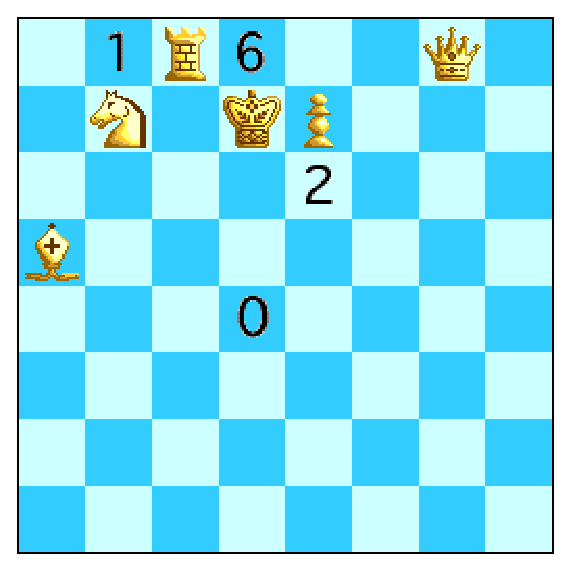
\includegraphics[width=0.4\textwidth]{figures/chessdemo.eps}
  \caption{An example puzzle with four numbered squares and its unique solution.}\label{fig:fig1}
\end{figure}

\section{Approach}
\subsection{Decision Variables}
The decision variables correspond to the coordinate pair of each piece. They are all
within the domain [0, 7] (inclusive). Furthermore, all of these coordinate pairs are
distinct both between each other, as well from the given numbered cells' coordinates.

\subsection{Constraints}
\subsubsection{All Distinct}
The first restriction placed is applied to the pieces' coordinates. It ensures that
no two pieces and/or numbered squares are placed in the same spot. To achieve
this we use the predicate \inlinecode{all\_distinct/1} with a list of the indexes of
each coordinate [X, Y]. An index corresponds to $Y * 8 + X$.

\subsubsection{Value}
The second set of restrictions is applied for each given cell, and it ensures that, its
value corresponds to number of attacking placed pieces. For this, the \inlinecode{value/3}
predicate is used. It first calculates a boolean value for each piece through the use of
the value predicate of its type, e.g.: \inlinecode{valueKing/3}. The returned value
corresponds to 1 if the piece is attacking the cell and to 0 if it isn't attacking.
We then constraint the sum of all these values to equal the value on the given
numbered square.

We always try to restrict the piece to attack the cell before restricting it to not attack.

\subsubsection{KingValue, KnightValue and PawnValue}
The predicates \inlinecode{valueKing/3}, \inlinecode{valueKnight/3}, \inlinecode{valuePawn/3}
restricts the given piece to attack a given square (returning 1) or not attack
(returning 0). The restrictions applied follow chess' rules: \textbf{King}
attacks squares orthogonally and diagonally adjacent; \textbf{Knight} attacks squares
in an \textit{L} pattern; \textbf{Pawn} attacks squares above it that are diagonally
adjacent.

\subsubsection{QueenValue, BishopValue and RookValue}
The predicates \inlinecode{valueQueen/4}, \inlinecode{valueBishop/4}, \inlinecode{valueRook/4}
behave similarly to the previously listed predicates, but also take into account
other pieces blocking it. This wasn't a problem in the previous predicates, because
they either only move a single square at a time (King, Pawn) or jump over other pieces
(Knight). Once again, chess rules tell us that, if not blocked, the rook can attack
horizontally and vertically, the bishop can attack diagonally, and the queen can attack
horizontally, vertically and diagonally.

The predicate \inlinecode{others\_is\_not\_between/3}, constraints whether or not the
path between the given piece and the target square is clear (no pieces blocking the path).
This predicate calls \inlinecode{is\_not\_between/3} for each other piece with a given
condition. This condition defines the path (diagonal, vertical or horizontal) between
the piece and its target square, e.g.: \inlinecode{[0, 0]-h-[3, 0]} is the path of
a piece in \inlinecode{[0, 0]} to \inlinecode{[3, 0]} horizontally. The predicate
\inlinecode{is\_not\_between/3} takes care of restricting the given piece to not
be the in the middle of the attack path (returning 1) (or the reverse). The predicate
\inlinecode{others\_is\_not\_between/3} uses this result to verify that all of the
members of the given list aren't in the attacking piece's path. If any other piece
blocks the attack path, this predicate yields 0.

\section{Solution Visualization}
The main (outermost) predicates that allow for a problem/solution visualization
are the \inlinecode{display\_board/1} and the \inlinecode{display\_board/2} predicates.

\subsection{The \inlinecode{display\_board(+NumberedSquares)} predicate}
This predicate will draw a chess board with the given numbered squares coordinates
showing the given values. This is used to show a problem without its solution. It
should be noted that the predicates used to visually represent a solution do so
"on-the-fly". This means that only the input data structures are used instead of
a \textit{game board} structure being generated and displayed.

The call \inlinecode{display\_board([[1, 0]-1, [3, 0]-6, [4, 2]-2, [3, 4]-0]).}
yields the following:
\begin{figure}[H]
  \centering
  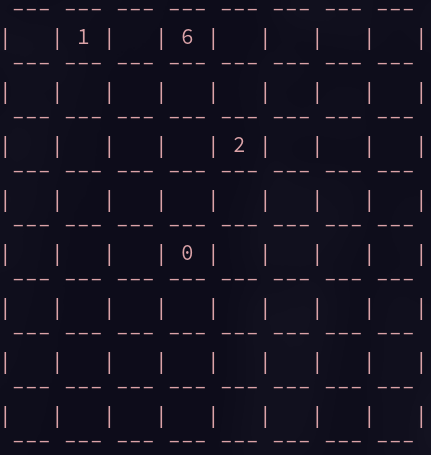
\includegraphics[width=0.4\linewidth]{figures/display_board_1.png}
  \caption{The textual representation of the puzzle show in figure\ref{fig:fig1}
  (without its solution).}\label{fig:fig2}
\end{figure}

\subsection{The \inlinecode{display\_board(+NumberedSquares, +Coords)} predicate}
Similarly to display\_board/1, this predicate will draw a chess board with the given
numbered cells. Along side those, the pieces in the given coordinates will also be
represented. The representation of each piece is as follows: King - \textbf{K},
Queen - \textbf{Q}, Rook - \textbf{R}, Bishop - \textbf{B}, Knight - \textbf{Kn},
and Pawn - \textbf{P}.

The call \inlinecode{display\_board([[1, 0]-1, [3, 0]-6, [4, 2]-2, [3, 4]-0],
[[3, 1], [6, 0], [2, 0], [0, 3], [1, 1], [4, 1]]).} yields the following:
\begin{figure}[H]
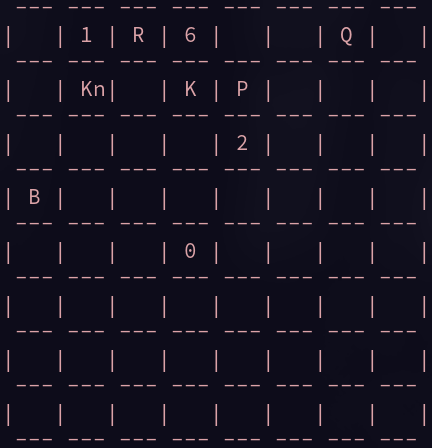
\includegraphics[width=0.4\linewidth]{figures/display_board_2.png}
  \centering
  \caption{The textual representation of the puzzle show in figure\ref{fig:fig1}
  (along side its solution).}\label{fig:fig3}
\end{figure}

\section{Problem generation}
The predicate \inlinecode{gen\_problem/3} was implemented to generated random
puzzles with the given number of numbered squares. This predicate starts by placing
the six chess pieces in random places on the board. Then, it runs the solver
to place the constraints for the given quantity of numbered cells. After posting
the constraints (labeling), we'll have a new puzzle. The puzzles generated also
show one of their solution (they can have more).

The puzzles generated have at least one solution, and the values for the decision
variables are selected randomly. In order to make puzzles more interesting
(in general), we've excluded the value 0 from the generated puzzles. The puzzles
generated avoid symmetries in the list of numbered squares by constraining the
numbered squares coordinates to be sorted (ascendantly) using their index ($Y * 8 + X$).
For example, \inlinecode{[[0, 0]-1, [1, 0]-2]} and \inlinecode{[[1, 0]-2, [0, 0]-1]}
are the same puzzle and thus, only the first is generated ($0 < 1$).

\begin{figure}[H]
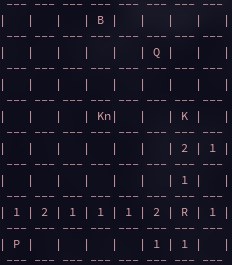
\includegraphics[width=0.3\linewidth]{figures/gen_problem.png}
  \centering
  \caption{Example run of puzzle/problem generation.}\label{fig:fig4}
\end{figure}

\section{Experiments and Results}
\subsection{Dimensional analysis}
\subsubsection{The impact of the quantity of numbered squares}
The more numbered squares the puzzle has, the longer it takes to solve it.

The problem in figure~\ref{fig:fig1} is the simplest problem we found with
an unique solution. Our solver finds that solution in about \textbf{0.02 seconds}.
From the problems in the puzzle's web page, this is the one that is solved
the fastest by our constraints.

This puzzle has four numbered squares, one of which has the value 6. This
is of note because, we always start constraining the pieces coordinates
in a that they can attack the given numbered square. A numbered square with
value 6 implies that all six pieces are attacking it, thus pruning the
possible coordinates for the pieces by a lot.

We can compare this puzzle to the following which also has a single solution,
but no numbered square with the value 6. It takes about \textbf{0.15 seconds} to
find the solution. This is significantly higher than the previous one
even though there are the same number of numbered squares.

\begin{figure}[H]
  \centering
  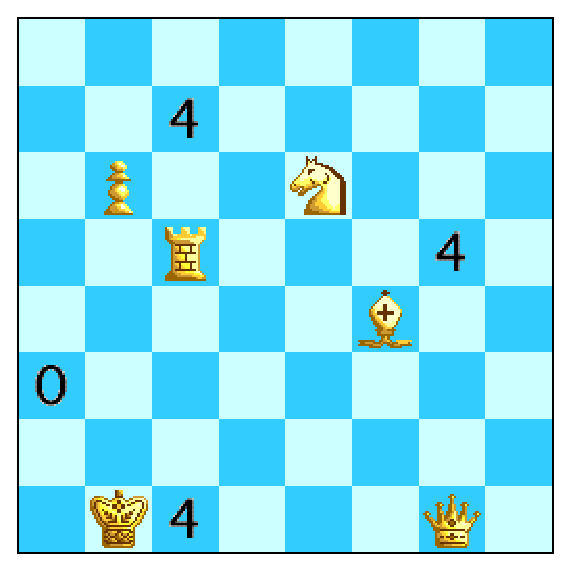
\includegraphics[width=0.4\linewidth]{figures/chess2.eps}
  \caption{A puzzle with four numbered squares and a unique solution.}\label{fig:fig5}
\end{figure}

\subsubsection{The special case for the value 0}
As previously stated, our constraints are posted aggressively on the attack
for each for each numbered square. This is very inefficient when the numbered
square we're dealing with has value 0 (no one can attack it). This led us to
create a special case for these numbered squares where we explicitly constraint
all pieces to not attack the numbered square from the get go, instead of
trying to attack it first. This change didn't affect the performance of puzzles
with little to no squares with 0 value.

The following example has a single solution and is solved much more quickly
than most puzzles with the same quantity of numbered squares, because of this
special case.

\begin{figure}[H]
  \centering
  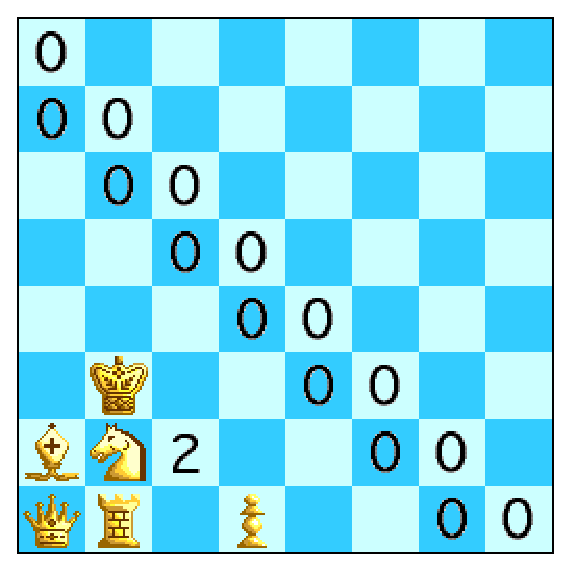
\includegraphics[width=0.4\linewidth]{figures/chess8.eps}
  \caption{A puzzle with four numbered squares and a unique solution.}\label{fig:fig6}
\end{figure}

\subsubsection{The processing order of numbered squares}
When trying new puzzles, we noticed that changing the order of the inputted
numbered squares, thus not changing the problem, but the processing order
of the squares, had an effect on the speed of discovering solutions. This
effect ranged from mild (a few fractions of a second) to extreme (one or two
hours).

The most extreme case we found was the following puzzle. This puzzle has a single
solution and the program was tacking hours to find it. By changing the order
the numbered squares are processed, we were able to reduce the processing time
to \textbf{under 8 seconds}.

\begin{figure}[H]
  \centering
  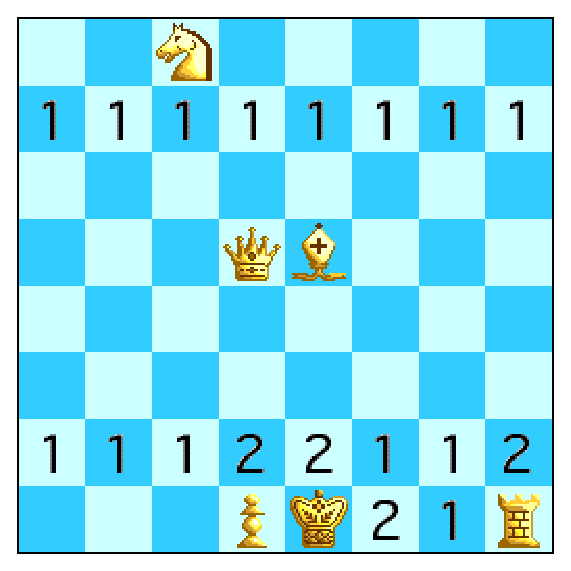
\includegraphics[width=0.4\linewidth]{figures/chess7.eps}
  \caption{A puzzle in which the order of the numbered squares processing makes a big impact.}\label{fig:fig7}
\end{figure}

This led us to believe that there should have been more focus on the preprocessing
of the numbered square list. As of now, we believe the best way to order the
processing of the squares is to order by the values from highest to the lowest.
After that, we disambiguate the ones with the same values by ordering
from the closest to the corners of the board to the ones closer to the center of
the board. Usually, this yields much better results, but not always. Sadly,
this means we aren't sure how to preprocess the numbered square list.

\subsection{Search strategies}
These performance tests were done on puzzle in figure~\ref{fig:fig7}. Each combination
of option was run three times. The numbers shown are the average of the three
attempts made for each option combination.

We decided to user \textbf{ffc} with \textbf{bisect}, because their performance
was was good in these tests and seemed to do also do well when testing other
puzzles. A close seconds was \textbf{ffc} with \textbf{median}. In this puzzle,
\textbf{occurrence} with \textbf{bisect} has a very good performance, but it
seems to be specific to this puzzle.

\begin{table}
  \begin{center}
    \caption{Search time for each option combination}
    \label{tab:table1}
    \begin{tabular}{l|c|c|c|c}
          & step & enum & bisect & median\\
      \hline
        leftmost        & 8.16s & 8.17s & 7.96s  & 8.14s  \\
      \hline
        min             & 8.29s & 8.20s & 7.82s  & 8.40s  \\
      \hline
        max             & 8.38s & 8.40s & 7.83s  & 8.60s  \\
      \hline
        ff              & 8.15s & 7.98s & 7.92s  & 8.08s  \\
      \hline
        anti\_first\_fail & 8.34s & 8.22s & 7.60s  & 11.15s \\
      \hline
        occurrence      & 7.82s & 7.75s & 7.41s  & 7.70s  \\
      \hline
        ffc             & 7.80s & 7.75s & 7.75s  & 7.76s  \\
      \hline
        max\_regret      & 8.15s & 7.91s & 7.84s  & 7.99s  \\
    \end{tabular}
  \end{center}
\end{table}

\section{Conclusions and Future Work}
The constraints implemented are able to find solutions to any problem fairly
quickly. Most times, lower quantities of numbered squares result in faster
solutions (less constraints). Numbered squares with values of 0 or 6 are
faster to take care of and problems with more of them are solved faster than
problems without (when comparing problems with the same quantity of numbered squares).

In the future, work should be focused in finding/implementing a way to do the
correct preprocessing of the numbered square list. This will ensure that the
implementation performs as fast as possible.

\begin{thebibliography}{8}
\bibitem{sicstusdocs}
    Sicstus Documentation
        \href{https://sicstus.sics.se/documentation.html}{https://sicstus.sics.se/documentation.html}.
        Last accessed 4 Jan 2021

\bibitem{slides}
    PLOG's PLR slides 
    \href{https://moodle.up.pt/pluginfile.php/60683/mod\_resource/content/10/PLR\%20SICStus.pdf}{https://moodle.up.pt/pluginfile.php/60683/mod\_resource/content/10/PLR\%20SICStus.pdf}
    . Last accessed 4 Jan 2021

\bibitem{puzzle}
    Chess Num Puzzle 
    \href{https://erich-friedman.github.io/puzzle/chessnum}{https://erich-friedman.github.io/puzzle/chessnum}
    . Last accessed 4 Jan 2021
\end{thebibliography}

\section{Annex}
\subsection{Graphs}
Note that the number above each bar represents the number of given cells of
its respective experience.

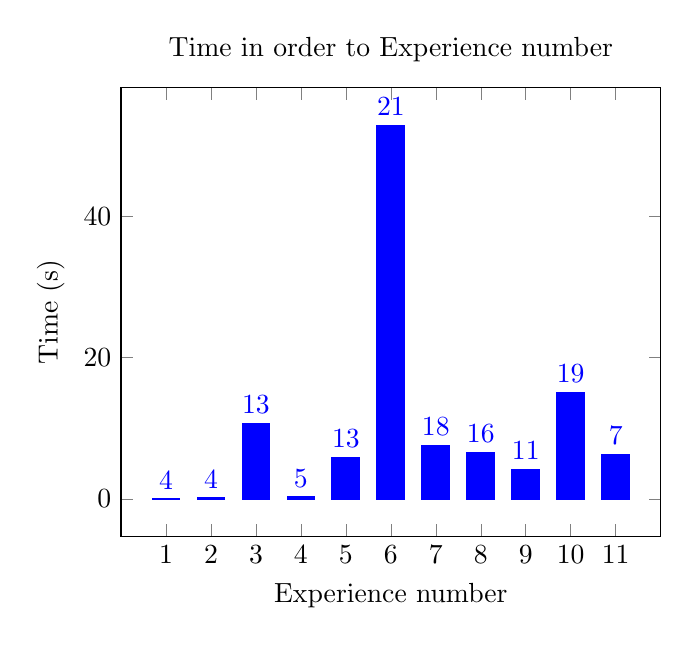
\begin{tikzpicture}
\begin{axis}[
    title={Time in order to Experience number},
    xlabel={Experience number},
    ylabel={Time (s)},
    xtick = data,
    grid style=dashed,
    nodes near coords
]
\addplot[
    ybar,
    fill=blue,
    point meta=explicit,
    color=blue
    ]
    coordinates {
        (1, 0.02) [4]
        (2, 0.15) [4]
        (3, 10.74) [13]
        (4, 0.31) [5]
        (5, 5.9) [13]
        (6, 52.91) [21]
        (7, 7.62) [18]
        (8, 6.59) [16]
        (9, 4.14) [11]
        (10, 15.11) [19]
        (11, 6.3) [7]
    };
\end{axis}
\end{tikzpicture}

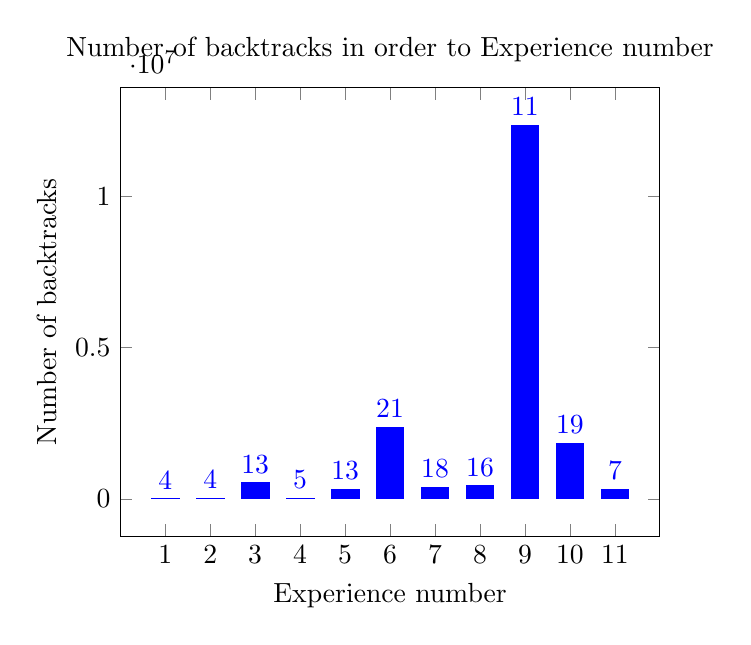
\begin{tikzpicture}
\begin{axis}[
    title={Number of backtracks in order to Experience number},
    xlabel={Experience number},
    ylabel={Number of backtracks},
    xtick = data,
    grid style=dashed,
    nodes near coords
]
\addplot[
    ybar,
    fill=blue,
    point meta=explicit,
    color=blue
    ]
    coordinates {
        (1, 870) [4]
        (2, 6423) [4]
        (3, 529728) [13]
        (4, 13458) [5]
        (5, 306581) [13]
        (6, 2374869) [21]
        (7, 389251) [18]
        (8, 423694) [16]
        (9, 12361393) [11]
        (10, 1823598) [19]
        (11, 302458) [7]
    };
\end{axis}
\end{tikzpicture}

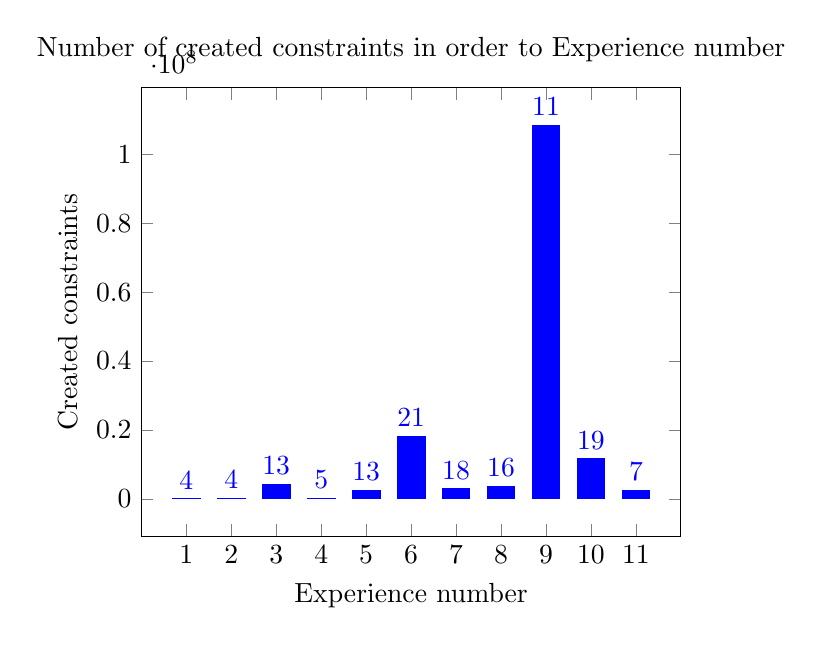
\begin{tikzpicture}
\begin{axis}[
    title={Number of created constraints in order to Experience number},
    xlabel={Experience number},
    ylabel={Created constraints},
    xtick = data,
    grid style=dashed,
    nodes near coords
]
\addplot[
    ybar,
    fill=blue,
    point meta=explicit,
    color=blue
    ]
    coordinates {
        (1, 7882) [4]
        (2, 59777) [4]
        (3, 4274679) [13]
        (4, 112229) [5]
        (5, 2464448) [13]
        (6, 18141558) [21]
        (7, 2925157) [18]
        (8, 3547552) [16]
        (9, 108464947) [11]
        (10, 11599568) [19]
        (11, 2379456) [7]
    };
\end{axis}
\end{tikzpicture}

\end{document}

%GRAPH DATA
%4 4 13 5 13 21 18 16 11 19 7
%1 - 0.02s
%Backtracks: 870
%Constraints created: 7882
%--------
%2newnew - 0.15s
%Backtracks: 6423
%Constraints created: 59777
%--------
%3new - 10.74s
%Backtracks: 529728
%Constraints created: 4274679
%--------
%4new - 0.31s
%Backtracks: 13458
%Constraints created: 112229
%--------
%5new - 5.9s
%Backtracks: 306581
%Constraints created: 2464448
%--------
%6 - 52.91s
%Backtracks: 2374869
%Constraints created: 18141558
%-----
%7new - 7.62s
%Backtracks: 389251
%Constraints created: 2925157
%--------
%8 - 6.59s
%Backtracks: 423694
%Constraints created: 3547552
%--------
%9new - 4.14s
%Backtracks: 12361393
%Constraints created: 108464947
%------
%10new - 15.11s
%Backtracks: 1823598
%Constraints created: 11599568
%----
%11new - 6.3s
%Backtracks: 302458
%Constraints created: 2379456
